\part{APLICACIÓN}

\section{Loopback digital}
	Tras la prueba del loopback analógico y del desarrollo de la interfaz I$^2$S, la  aplicación más sencilla que probaba esto último es un loopback digital. Gracias a cómo se ha desarrollado el codec, el desarrollador de aplicaciones no tiene que preocuparse cuando tiene que coger y soltar los datos de audio si el procesamiento de audio es sólo combinacional como es el caso.
	Una mínima modificación de la aplicación permite hacer un cruze de canales que ayudó a cerciorarnos de que el audio era procesado exclusivamente por la FPGA. Posteriormente esta aplicación será modificada dándonle el nombre de \emph{ATTENUATOR$\_$6dB} para convivir con \emph{REVERB$\_$COMB}, se explica debajo en \ref{directo:attenuator-loopback}

\section{Reverb COMB}
\begin{figure}[h]
\begin{center}
	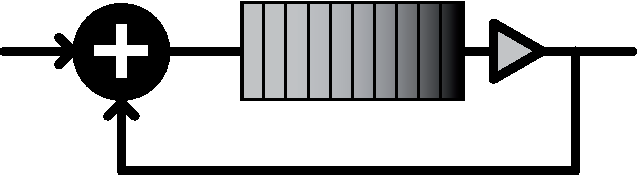
\includegraphics[width=0.7\textwidth]{./reverb_simple_diagram-eps-converted-to}
\caption{Diagrama de una reverb basada en los rebotes del sonido entre dos paredes}
\end{center}
\end{figure}
	Este flujograma tiene una respuesta en frecuencia parecida a la forma de un peine, es decir, deja pasar con facilidad unas componentes de frecuencia (púas del peine) y otras no tanto (valles del peine). El número de picos y la distancia entre ellos (equiespaciados entre entre 0 y $\pi$) depende del tiempo entre rebotes, lo que en el mundo digital es el número de muestras de retardo. Vemos que el esquema contiene los tres bloques básicos de cualquier DSP: un sumador, un multiplicador y una memoria.
	
\paragraph{} Se pensó en otros flujogramas más complejos como inlcuir un filtro paso bajo en la red de realimentación que ayuda a suavizar el sonido metálico, pero los pocos recursos de la FPGA y que tal sonido una vez llevado a la FPGA no era tan evidente como mostraba Matlab lo hicieron desaconsajable. (¿ponemos las figuras?).
\paragraph{Algoritmos de punto fijo} Para estudiar el algoritmo y poder dimensionar los parámetros de retardo y atenuación utilizamos en Matlab. El problema radica en que Matlab usa algoritmos en coma flotante que en un FPGA no están soportados de forma nativa. Así que tuvimos que rediseñar nuestro problema a uno de punto fijo definiendo el ancho de palabra en cada segmento del flujograma tal y como se puede apreciar en esta imagen:

\begin{figure}[h]
\begin{center}
	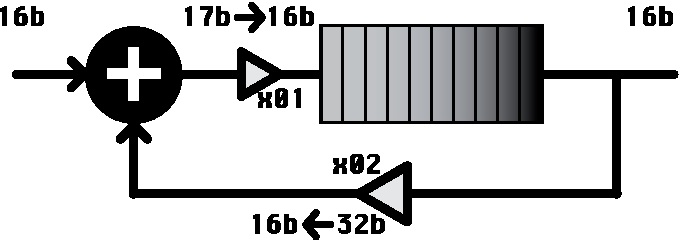
\includegraphics[width=0.7\textwidth]{./reverb_implemented_diagram-eps-converted-to}
\caption{Anchos de palabra asignados a la aplicación}
\label{default}
\end{center}
\end{figure}

	En principio se trabajo con la máxima resolución posible (20 bits), pero con ánimo de reservar los máximos recursos a la memoria se decidió por recortar el número de bits de 20 a, en un principio, 12. Pero al ver los informes del ISE, vimos que como usa las LUTs para almacenar y éstas son unas ROM de 4 entradas (16 bits) la diferencia en recursos entre 12 y 16 debía ser nula.
	
\paragraph{Restricciones adoptadas} 
	Por la falta de conocimientos en Matlab acerca del punto fijo y el desconocimiento de la estadística de las señales que permite saber si ciertos bits de la palabra se usan y con que frecuencia, utilizamos unas restricciones poco maduradas debido a la escasez de tiempo y al poco manejo práctico que tenemos de la \emph{coma} en el mundo digital, son las siguientes:
\begin{itemize}
\item \textbf{Sumador}: la suma de dos palabras de X bits, podría resultar una palabra de X+1 bits, cómo la memoria tiene Y filas de X bits, tenemos que decidir si truncamos la palabra o sí la redondeamos a su valor más proximo, en el caso que pensemos en el lugar donde está la \emph{coma} . 
	Se decidió por truncar cogiendo los bits más significativos, como resultado obtenemos una división por un factor 2 (multiplicador x01)  
\item \textbf{Memoria}: el elemento más delicado de la aplicación, define los bits que se entregan al codec para su reproducción.
\item \textbf{Multiplicador}: Implementado como un multiplicador por una constante, tiene dos entradas de X bits y la salida es de 2X bits de los cuales sólo X se pueden aprovechar.  La constante multiplicadora tiene que ser menor que 2 para que no haya inestabilidades, ya que la atenuación total será el factor de multiplicación de este multiplicador entre 2, debido al efecto del sumador. 
	La señal entregada por el codec asumimos que es sin decimales, al multiplicarla por una constante con X-1 decimales, nos queda al final una palabra de 2X bits de los cuales X-1 son decimales, X son la parte entera (el MSB representa el signo) y nos queda otro bit (el MSB de la palabra de 2X bits) que extiende este signo.
	Cogemos la parte entera, sin tener en cuenta la parte decimal que nos serviría para aproximar.
\end{itemize}
 
	\subsection{Retardo}
	Por la escasez de recursos se convierte en el módulo más complicado de la aplicación hay dos formas de implementarla siendo la segunda la más adecuada  
		\subsubsection{Registros en cadena}
		Esta forma de implementación es la más sencilla e ineficaz a la vez, consiste un registro de desplazamiento de ancho la palabra de audio. Ocupa mucha área (recursos y cableado) y tiene un gasto importante de potencia ya que en cada flanco de reloj se mueven todos los datos.
		VHDL lo infiere si se hace explicitamente el desplazamiento:
		\begin{verbatim}
		type arr is array(0 to samples_delay-1) 
		                  of std_logic_vector (11 downto 0); 
		signal delayer : arr;
		...
		FOR i IN 0 TO samples_delay-2 LOOP
			delayer(i+1) <= delayer(i);
		end loop;
		\end{verbatim}

		
		\subsubsection{RAM}
		Esta forma de inferir el retardo es la más adecuada ya que utiliza recursos de la placa específicos para ella (blocks ram, ram distribuida..), la forma de inferirla es como si accediéramos a un array, por lo tanto necesitamos un puntero y algo que controle el valor del puntero. Como leemos y escribimos en un flanco de reloj el ISE infiere una RAM de X*Y de doble puerto, aunque como las direcciones que leemos y escribimos es la misma, sólo utiliza un puerto en la conexión. 
		\begin{verbatim}
		type arr is array(0 to samples_delay-1) 
		                   of std_logic_vector ((bits-1) downto 0); 
		signal delayer : arr;
		...
		OUTPUT_TEMP <= delayer(index);									
		delayer(index) <= OUTPUT_SUM(bits DOWNTO 1);															
		if index < (samples_delay-1) then				
			index <= index + 1;
		else
			index <= 0;
		end if;
	

\end{verbatim}


	\subsection{Atenuación en el lazo de realimentación} \label{directo:attenuator-loopback}
		Al pasar el algoritmo a coma fija, se hace una división por un factor 2 al truncar y elegir los bits más significativos. Si la \emph{reverb} está en un canal y en el otro un loopback digital, este último canal sonaría el doble de fuerte en tensión (6dB en potencia) haciendo aún más imperceptible la reverberación, por lo tanto se aplica la misma atenuación en el loopback para normalizar el volumen en los dos canales.

		\subsubsection{Directo} 
		Aunque el lazo de realimentación no tenga atenuación la \emph{reverb} no es inestable al tener una atenuación implícita después del sumador (truncamiento y elección de los bits). Esta fue la primera implementación y lo que motivo la modificación del \emph{loopback digital} a \emph{attenuator$\_$6dB}.
		
		\subsubsection{Multiplicador}
		Una mejora significativa es la introducción de un multiplicador en el lazo. Las entradas de este multiplicador son \emph{STD$\_$LOGIC$\_$VECTOR} usando la librería \emph{IEEE.STD$\_$LOGIC$\_$SIGNED.ALL} nos permite hacer multiplicaciones con signo. Nos quedan dos bits de signo al usar una entrada con un bit de parte entera y los restantes la parte decimal. El ISE infiere un multiplicador por una constante que tendrá menos área que uno con las dos entradas a priori desconocidas.

	



